\section{Aprendizaje de sistemas basados en reglas con Programación Genética}

De cara al descubrimiento de reglas utilizando Programación Genética existen algunos problemas, así como diversos enfoques y tomas de decisiones a realizar. En esta sección comentaremos dichos problemas, discutiremos las posibles soluciones, así como analizar las distintos enfoques que se pueden tomar, además de realizar una comparación entre todos estos detalles. Aunque a lo largo de la década de los noventa y a principios de siglo se han realizado las distintas propuestas de cara a este ámbito, Alex A. Freitas \cite{dataMiningDescubrimientoReglasGeneticos} realizó una recopilación y discusión sobre este ámbito, que será la que utilizaremos de base.


\subsection{El problema de la clausura en Programación Genética}

Uno de los problemas de utilizar Programación Genética para aprender reglas es que, al representar reglas en forma de árboles, podemos llegar a tener reglas que no tienen sentido debido a los distintos tipos de nodos utilizados dentro del árbol.

De cara a solucionar este problema habitualmente en la literatura se proponen tres posibles soluciones:

\begin{enumerate}
	\item Binarizar todos los símbolos terminales y utilizar solo funciones booleanas: Transformar todos los tipos de nodos a un solo tipo.
	\item Añadir restricciones a Programación Genética y tener en cuenta dichas restricciones al implementar el algoritmo.
	\item Utilizar un algoritmo de Programación Genética basado en gramáticas.
\end{enumerate}

\subsubsection{Binarizar los símbolos terminales}

Esta solución es la más simple de todas. Se basa en, todas las posibles operaciones, reducirlas a un único nodo que puede tomar valores verdadero o falso, de forma que podamos combinar todos los nodos de operaciones lógicas con los nodos terminales de funciones booleanas.

Un ejemplo de esto sería, teniendo un caso donde tenemos un atributo color, convertir la estructura $Color = AZUL$, de un árbol donde el nodo raíz es $=$, el hijo de la izquierda es $Color$ y el de la derecha $AZUL$, a un único nodo $Color = AZUL$ en el problema, de forma que el algoritmo de Programación Genética trabaje con estas funciones booleanas como nodos terminales.

\begin{figure}[H]
    \centering
	 \begin{subfigure}[b]{0.49\textwidth}
		 \centering
		 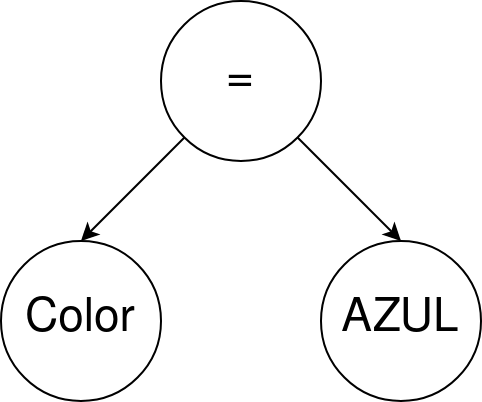
\includegraphics[width=0.5\textwidth]{arbol_color_azul.png}
		 \caption{Representación original de una igualdad expresada en un árbol.}
		 \label{fig:arbol_color_azul}
	 \end{subfigure}
	 \begin{subfigure}[b]{0.49\textwidth}
		 \centering
		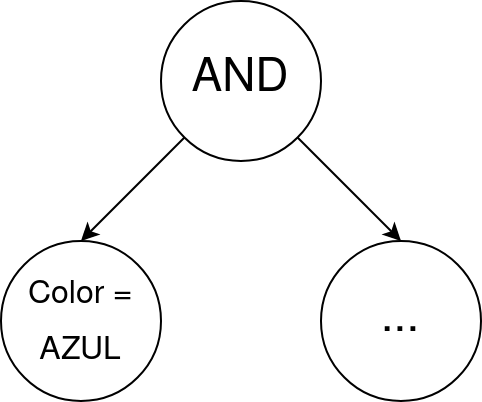
\includegraphics[width=0.5\textwidth]{arbol_funcion_booleana.png}
		\caption{Representación binarizando a funciones binarias los nodos terminales.}
		\label{fig:arbol_funcion_booleana}
   \end{subfigure}
	\caption{Ejemplo de binarización de una expresión a una función binaria.}
	\label{fig:arbol_exp_a_funcion_booleana}
\end{figure}


Un problema de este enfoque es que hay que adaptar el conjunto de datos de entrada y hacer un preprocesamiento para crear estas funciones lógicas, de forma que de cada atributo categórico podríamos generar $2^n$ funciones lógicas por cada operador que se pueda aplicar a dicho atributo, mientras que para los atributos continuos tenemos que añadir una forma de modificar las constantes de dichas funciones booleanas.

Otro detalle si se utiliza esta solución es que sigue sin resolver el problema de restricciones semánticas, es decir, aunque se trabajen con funciones binarias, podrías seguir encontrando el siguiente caso:

\begin{figure}[H]
    \centering
	  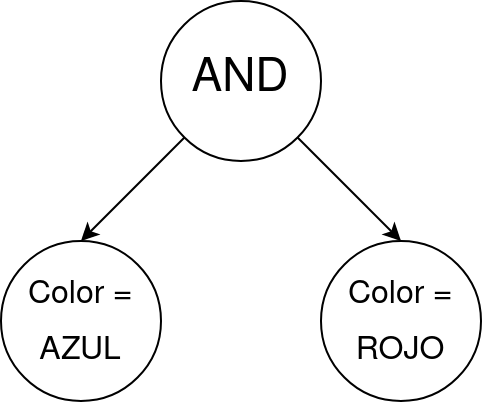
\includegraphics[scale = 0.3]{arbol_problema_restriccion_semantica.png}
    \caption{Árbol incorrecto desde el punto de vista semántico.}
	 \label{fig:arbol_problema_restriccion_semantica}
\end{figure}

Aunque este problema en principio no nos debería preocupar, porque al aprender un modelo de Programación Genética si se llega a este caso la regla no tendrá una buena puntuación, ya que no representará a ninguna observación.

\subsubsection{Añadir restricciones sintácticas a Programación Genética}

En este caso, en lugar de modificar las funciones utilizadas por Programación Genética para construir el árbol, se añaden restricciones a cada nodo.

Al lanzar el algoritmo se incluirá información de, para un tipo de nodo, qué tipo de nodos pueden ser usados como hijos de dicho nodo. Esto permite evitar situaciones donde, por ejemplo, se genere un operador de comparación como hijo de otro operador de comparación.

A este tipo de algoritmos de Programación Genética se les llama Strongly-Typed GP (STPG), ya que lo que realmente estamos haciendo es una restricción de tipos a los nodos.

Este tipo de aproximaciones se basan en las siguientes reglas para generar árboles correctos:

\begin{itemize}
	\item El nodo raíz devuelve el mismo tipo de dato del requerido por el problema (un valor booleano si estamos aprendiendo reglas, o un número real si se está haciendo regresión simbólica).
	\item Cada nodo devuelve el mismo tipo de dato que el tipo marcado por su nodo padre en sus argumentos.
\end{itemize}

Siguiendo estas dos reglas intuitivas conseguimos construir árboles correctos, pero es cierto que tenemos que tener en cuenta estas restricciones a la hora de implementar los operadores de Programación Genética, en especial el operador de cruce. La única restricción que añadiría este enfoque es que al operar con los árboles se escojan siempre nodos que tienen el mismo tipo de dato necesario en sus padres. Por ejemplo, en el operador de cruce, al cruzar dos individuos, si escogemos dentro del primer hijo un nodo que genera un valor de tipo $T_1$, es necesario que el nodo escogido del segundo hijo con el que se va a cruzar también genere un valor de tipo $T_1$, de forma que al intercambiarlos de árbol los nodos padres no seleccionados sigan cumpliendo las restricciones.


\subsubsection{Programación Genética basada en gramáticas}

Por último, otro de los enfoques, y también uno de los más utilizados, es utilizar una gramática al generar los árboles. Este enfoque es una modificación de añadir restricciones al algoritmo de Programación Genética, donde las restricciones semánticas y sintácticas las impone una gramática.



\subsection{Representación de la población}

Normalmente en los algoritmos evolutivos se suele representar a un individuo como una solución al problema, de forma que la población explore el conjunto de soluciones buscando la mejor. Sin embargo, para aprender reglas tenemos distintas opciones, dependiendo de si consideramos una solución a un conjunto de reglas que clasifiquen el conjunto de datos completo, o si interpretamos como solución las reglas de forma individual.

Por este motivo, aparecen dos enfoques distintos, dependiendo de la representación de los individuos.

\subsubsection{Enfoque Pittsburgh}

El enfoque Pittsburgh se basa en representar un individuo de la población como un conjunto de reglas completo, por lo tanto, un individuo de la población representa una solución completa al problema.

La principal ventaja de utilizar este esquema es que un individuo puede tener en cuenta el conjunto de reglas completo, de forma que se tenga en cuenta cuando dos reglas se solapan, o si es posible reducir reglas redundantes, cosa que, como veremos en la siguiente sección, no es posible con el enfoque Michigan.

Otra ventaja de este enfoque es que la función de ajuste tiene en cuenta todo el conjunto de reglas, no como de buenas son las reglas de forma individual, lo que puede ayudar a una mayor generalización en las soluciones y evitar el sobreajuste.

\subsubsection{Enfoque Michigan}

Por otro lado, el enfoque Michigan se basa en representar un individuo como una única regla, de forma que un individuo solo representa una solución parcial al problema, ya que solo servirá para ciertas observaciones del conjunto de datos.

Dentro de este enfoque, para construir una solución completa al problema, existen dos formas de proceder:

\begin{enumerate}
	\item Lanzar múltiples veces el algoritmo evolutivo, para obtener así múltiples reglas que solucionen el problema.
	\item Utilizar la población completa del algoritmo como solución al problema.
\end{enumerate}

Como podemos imaginar, la primera opción se puede utilizar dividiendo el conjunto de datos por clase, de forma que cada algoritmo evolutivo se centre en aprender reglas para dicha clase, y por tanto lanzando tantas veces el algoritmo como clases tenemos en el problema.

Con la segunda opción tenemos la ventaja de lanzar una única vez el algoritmo, sin embargo hay que tener en cuenta que se deben introducir mecanismos de diversidad para que la población no se estanque y simplemente clasifique reglas de la clase mayoritaria, o elimine reglas más especificas que otras por el simple hecho de cubrir una zona más pequeña del espacio, pero tal vez más interesante.



\newpage
